% Copyright (c) 2015 Benito Palacios Sánchez - All Rights Reserved.
% Esta obra está licenciada bajo la Licencia Creative Commons Atribución 4.0
% Internacional. Para ver una copia de esta licencia, visita
% http://creativecommons.org/licenses/by/4.0/.

% Template
\documentclass{beamer}

% Font
\usepackage[T1]{fontenc}                % Output font
\usepackage[utf8]{inputenc}             % Input encoding
\usepackage[spanish,es-tabla]{babel}    % For Spanish texts
\usepackage{FiraSans}

% Theme
\usetheme{Frankfurt}
\usecolortheme{whale}

% My package
\usepackage{Layout}

% Information about author and document
\title{Mecanismos de protección de datos en videojuegos}
\date[2015]{Julio de 2015}
\author{Benito Palacios Sánchez}
\institute[ETSIIT - UGR]
{Escuela Técnica Superior de Ingenierías Informática y Telecomunicación\\
  Universidad de Granada
}

\begin{document}

    % Copyright (c) 2015 Benito Palacios S�nchez - All Rights Reserved.
% Esta obra est� licenciada bajo la Licencia Creative Commons Atribuci�n 4.0
% Internacional. Para ver una copia de esta licencia, visita
% http://creativecommons.org/licenses/by/4.0/.

\chapter{Introducci�n}

    % Copyright (c) 2015 Benito Palacios Sánchez - All Rights Reserved.
% Esta obra está licenciada bajo la Licencia Creative Commons Atribución 4.0
% Internacional. Para ver una copia de esta licencia, visita
% http://creativecommons.org/licenses/by/4.0/.

\section{Introducción}
\subsection{}

\begin{frame}{Motivación}
\begin{columns}
    \begin{column}{0.5\textwidth}
    \begin{wideitemize}
        \item<1-> Los videojuegos son una clave de nuestra cultura actual.

        \item<2-> Su industria es la segunda con más ganancias.

        \item<3-> Preocupación por protección anti-copias, derechos de autor, trampas.
    \end{wideitemize}
    \end{column}

    \begin{column}{0.5\textwidth}
        \only<1>{
            \includefigure{Estadísticas sobre jugadores en EE. UU. \scriptsize{}Fuente: \url{http://www.esrb.org} (2010).}{imgs/gamer_stats.png}
        }

        \only<2->{
            \includefigure{Estadísticas sobre la industria de videojuegos en EE. UU. \scriptsize{}Fuente: \url{http://www.esrb.org} (2009).}{imgs/game_ind_stats.png}
        }
    \end{column}
\end{columns}
\end{frame}

\begin{frame}{\textit{ROM Hacking}}
    \begin{block}{Ingeniería inversa}
        La ingeniería inversa es el proceso de analizar un sistema para identificar sus componentes y relaciones y, crear una representación del sistema en otro formato o a un nivel más alto de abstracción.
    \end{block}

    \begin{block}{\textit{ROM Hacking}}<2->
        Ingeniería inversa sobre videojuegos. El nombre viene realizar modificaciones (\textit{hacks}) sobre juegos que suelen distribuirse en memorias de solo lectura (\textit{Read Only Memory}).
    \end{block}
\end{frame}


    % Copyright (c) 2015 Benito Palacios Sánchez - All Rights Reserved.
% Esta obra está licenciada bajo la Licencia Creative Commons Atribución 4.0
% Internacional. Para ver una copia de esta licencia, visita
% http://creativecommons.org/licenses/by/4.0/.

\section[Fan-traducciones]{Traducciones no oficiales}
\subsection{Saga Pokémon}
\begin{frame}{Saga Pokémon}

\end{frame}

\begin{frame}{Metodología}
\end{frame}

\begin{frame}{Pokémon Perla y Diamante}

\end{frame}

\begin{frame}{Pokémon HeartGold y SoulSilver}

\end{frame}

\begin{frame}{Pokémon Blanco y Negro}

\end{frame}

\begin{frame}{Pokémon Conquest}

\end{frame}

\subsection{Ninokuni: El Mago de las Tinieblas}
\begin{frame}{Ninokuni: El Mago de las Tinieblas}

\end{frame}

    % Copyright (c) 2015 Benito Palacios Sánchez - All Rights Reserved.
% Esta obra está licenciada bajo la Licencia Creative Commons Atribución 4.0
% Internacional. Para ver una copia de esta licencia, visita
% http://creativecommons.org/licenses/by/4.0/.

\section[Contenido con copyright]{Contenido con derechos de autor}
\subsection{Libros electrónicos}
\begin{frame}{Ninokuni}

\end{frame}

\begin{frame}{100 Classic Book Collection}

\end{frame}

\subsection{Bandas sonoras}
\begin{frame}{Guitar Hero: On Tour}

\end{frame}

\begin{frame}{Duet}

\end{frame}

    % Copyright (c) 2015 Benito Palacios Sánchez - All Rights Reserved.
% Esta obra está licenciada bajo la Licencia Creative Commons Atribución 4.0
% Internacional. Para ver una copia de esta licencia, visita
% http://creativecommons.org/licenses/by/4.0/.

\section{Servicios en línea}
\subsection{Multijugador}
\begin{frame}[fragile]{Captura de paquetes}
\begin{columns}

\begin{column}{0.35\textwidth}
Estrategia \textit{man-in-the-middle}
\begin{center}
    \includefigure{\textit{Man-in-the-middle}}{imgs/man_middle.eps}
\end{center}
\end{column}

\begin{column}{0.5\textwidth}
\uncover<2->{Modificación DeSmuME.}
\begin{itemize}
    \item<3-> Paquetes PCAP.
\end{itemize}
\begin{uncoverenv}<3->\begin{lstlisting}
void create_packet();
void save_packet(u8* packet,u32 len);
void save_adhocPacket(u8* packet,
  u32 len, void* addr, bool isSent);
\end{lstlisting}\end{uncoverenv}

\begin{itemize}
    \item<4-> Exportar paquetes.
\end{itemize}
\uncover<5->{\scriptsize\texttt{HandleDebugEvent\_Execute()} en \texttt{debug.cpp}.}
\vfill
\visible<6->{\includefigure{\textit{RC4Finder.}}{imgs/rc4finder.png}}
\end{column}

\end{columns}
\end{frame}

\begin{frame}{Servidores para Nintendo DS}

\begin{center}
    \visible<2->{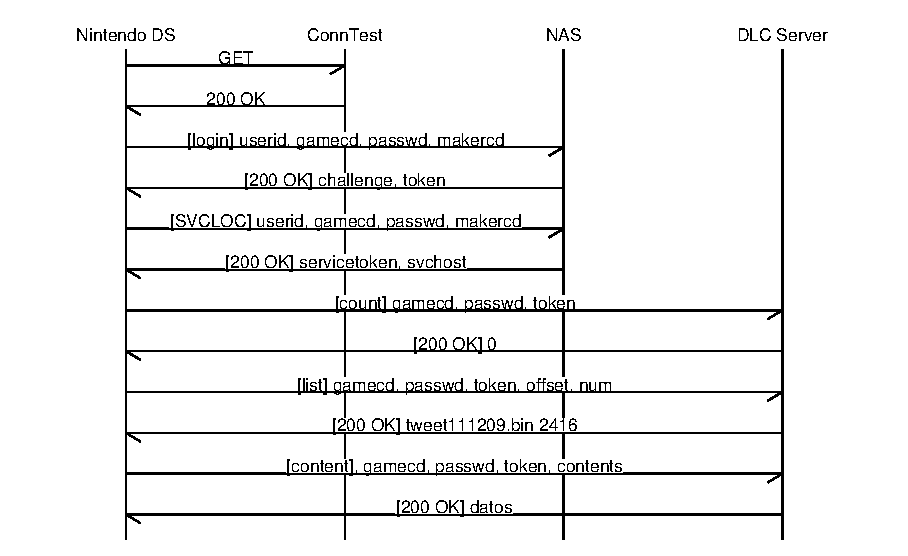
\includegraphics[width=\textwidth,height=0.5\textheight,keepaspectratio]{imgs/nds_dwc.eps}}
\end{center}

\uncover<3->{Vulnerabilidades:}
\begin{columns}
\footnotesize
\begin{column}{0.3333\textwidth}
    \begin{itemize}
        \item<4-> Puerto 80 del NAS abierto.
    \end{itemize}
\end{column}
\begin{column}{0.3333\textwidth}
    \begin{itemize}
        \item<5-> Contraseña no usada.
    \end{itemize}
\end{column}
\begin{column}{0.3333\textwidth}
    \begin{itemize}
        \item<6-> Autenticación simple.
    \end{itemize}
\end{column}

\end{columns}
\end{frame}

\begin{frame}{Preguntados}
\begin{columns}
    \begin{column}{0.15\textwidth}
        
\includegraphics[width=\textwidth,keepaspectratio]{imgs/preguntados_logo.png}
    \end{column}
    \begin{column}{0.85\textwidth}
        Trivial para plataformas móviles.
    \end{column}
\end{columns}

\vfill
\vspace{0.35cm}
\uncover<2->{Vulnerabilidades:}
\begin{columns}
    \begin{column}{0.5\textwidth}
    \begin{itemize}
        \item<3-> Comunicación HTTP.
    \end{itemize}
    \end{column}

    \begin{column}{0.5\textwidth}
    \begin{itemize}
        \item<4-> Solución enviada antes de preguntar.
    \end{itemize}
    \end{column}
\end{columns}

\only<4>{\includefigure{Preguntas, respuesta y solución de una partida}{imgs/preguntados_hack.png}}

\only<5>{\includefigure{Preguntas, respuesta y solución de una partida}{imgs/preguntados_hack_question.png}}

\only<6>{\includefigure{Preguntas, respuesta y solución de una partida}{imgs/preguntados_hack_answer.png}}

\end{frame}

\subsection{Contenidos descargables}
\begin{frame}{Duet}
\begin{center}
\includegraphics[width=0.15\textwidth,keepaspectratio]{imgs/duet_logo.png}\end{center}

\begin{columns}
    \begin{column}{0.5\textwidth}
    \begin{itemize}
        \item<2-> Niveles extras por 0,99€.
        \item<4-> BD con preferencias sin proteger.
        \note<1>[item]{Es SQLite y se puede usar software como SQLiteMan}
    \end{itemize}
    \end{column}

    \begin{column}{0.5\textwidth}
    \begin{itemize}
        \item<3-> Ya incluídos pero desactivados.
        \item<5-> Se puede activar a mano.
    \end{itemize}
    \end{column}
\end{columns}

\visible<5->{\includefigure{Filas con estado de los contenidos extras}{imgs/duet-levels.png}}

\end{frame}

\begin{frame}{\textit{Download Play}}
Compartir demos con comunicación inalámbrica ad-hoc.
\vfill
\uncover<2->{\underline{Problema:}}
\begin{itemize}
    \item<3-> Envío de código de una consola a otra.
    \item<4-> El código principales se firman con \texttt{RSA}.
\end{itemize}
\vfill
\uncover<5->{\underline{Solución de Nintendo:}}
\begin{itemize}
    \item<6-> Comprobar integridad con \texttt{HMAC}.
    \item<7-> Solo si con \textit{Download Play}.
\end{itemize}
\end{frame}


    % Copyright (c) 2015 Benito Palacios S�nchez - All Rights Reserved.
% Esta obra est� licenciada bajo la Licencia Creative Commons Atribuci�n 4.0
% Internacional. Para ver una copia de esta licencia, visita
% http://creativecommons.org/licenses/by/4.0/.

\chapter{Metodolog�a}
\label{sec:met}
Este cap�tulo explicar� las diferentes metodolog�as llevadas a cabo durante la realizaci�n del proyecto.
No existe un m�todo �nico a la hora de realizar un trabajo de ingenier�a inversa, cada juego es diferente, programado por diferentes compa��as en distintos instantes de tiempo.
Al trabajar con formatos, estos van evolucionando, a�adiendo m�s campos o siendo reemplazados por nuevos con mayor funcionalidad.
Analizando instrucciones m�quina, estas cambian en cada compilaci�n del juego, especialmente los registros usados.
Aunque la funcionalidad del c�digo sea la misma, problablemente no se usen los mismos registros, valores de pila, haciendo dif�cil poder reconocer un mismo algoritmo en dos juegos distintos.

El objetivo de las siguiente secciones es mostrar qu� t�cnicas, programas y pasos se han realizado a la hora de analizar los juegos de este trabajo.
Apartir de ellos, y con peque�as modificaciones, se pueden analizar aspectos de seguridad para otro conjunto de videojuegos.

\section{An�lisis de ficheros}
Una vez decidido un juego objetivo se debe reunir informaci�n sobre �l.
Conocer el desarrollador, el a�o de lanzamiento y g�nero del juego pueden ser �tiles pues, proporcionan indicios sobre el tipo de ficheros que contiene.
Usando programas de exploraci�n de ficheros como Tinke\footnote{\url{https://github.com/pleonex/tinke}}, se pueden reconocer los tipos de formato est�ndar y comenzar a trabajar sobre ellos.

El inter�s sin embargo es analizar aquellos formatos nuevos, que codifican recursos como im�genes y textos.
Los nombres y directos de los archivos son la primera referencia sobre el tipo de contenido.
Por ejemplo, tomando el juego de \textit{Ninokuni} para \acl{NDS}, el archivo \texttt{/data/UI/Menu/Skin/2/CheckShee\allowbreak{}t/bg\_a.n2d} debe contenido elementos de la interfaz gr�fica (\textit{UI}) del men� (\textit{Menu}) del juego.
Adem�s, la abreviatura \textit{bg} se utiliza para describir im�genes de fondo de pantalla (\textit{background}).
Mirando el contenido de este archivo con un visor hexadecimal se puede ver en la posici�n \texttt{0x54} se encuentran los caracteres \texttt{RLCN}, correspondientes a la cabecera de un formato est�ndar en la \acl{NDS} (Figura~\ref{fig:met-bg1}).

\includefigure{fig:met-bg1}{Contenido de un fichero con im�genes de \textit{Ninokuni}.}{imgs/MET-Bg1.png}

Al contrar esa cabecera, indica que este archivo contiene varios ficheros, en un formato similar a \texttt{zip}.
El an�lisis se centrar�a en saber c�mo extraer los ficheros para luego determinar qu� datos tienen cada uno de ellos.
Como dato indicativo se tiene que los datos del primer fichero empiezan en la posici�n \texttt{0x54}, por lo que habr� que buscar un valor qu� indique esta posici�n.
En la posici�n \texttt{0x0C}, se observa justo ese valor, seguido de \texttt{0x228}.
Frecuentemente, despu�s de la posici�n de un fichero se indica su tama�o, por lo que habr� que comprobar si el primer fichero termina en la posici�n \verb!0x54 + 0x228 = 0x27C!. En la Figura~\ref{fig:met-bg2} se ve que en esa posici�n aparece la cabecera \texttt{RGCN}, est�ndar para otro formato de archivo.

\includefigure{fig:met-bg2}{Contenido de un fichero comprimido de \textit{Ninokuni}.}{imgs/MET-Bg2.png}

Esto corrobora la estructura que se intu�a, por lo que por cada fichero hay 8 bytes indicando posici�n y tama�o.
Para determinar el n�mero de ficheros se puede calcular cuantos archivos especifica esa \textit{tabla de contenidos}, restando el principio del primer fichero a la posici�n de la primera entrada y diviendo por el n�mero de bytes dedicado a cada fichero: \verb!(0x54 - 0x0C) / 0x08 = 9!.
El resultado es que se han especificado 9 ficheros, valor que coincide con el encontrado en la posici�n \texttt{0x08} (Figura~\ref{fig:met-bg1}).

Esta forma de razonar es la que se ha empleado para averiguar de los formatos estudiados en el trabajo.
Faltar�a averiguar el contenido de cada fichero.
Estudiando los formatos m�s comunes, se puede identificar (Figura~\ref{fig:met-bg2}) que al principio hay colores, pues cada valor de 16 bits est� pr�ximo al siguiente.
Al final hay informaci�n sobre cada p�xel, �ndice al color de la paleta, pues se repiten muchos valores que est�n pr�ximos, esto concuerda con el hecho de que un p�xel en una imagen suele tener a su alrededor p�xeles de similar color.

Otro ejemplo se encuentra en los archivos de tipo \texttt{PSAR} (Figura~\ref{fig:met-psar}) analizados en la Secci�n~\ref{sec:cr-nino}.
En ellos, en la posici�n \texttt{0x08}, mediante los caracteres \texttt{ASCII} se indica el tipo de compresi�n que se usa sobre los datos, \texttt{zlib}.

\begin{figure}[bh]
\centering
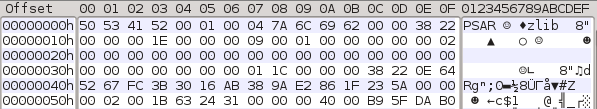
\includegraphics{imgs/CR-PSAR.png}
\caption{Primeros bytes del fichero \texttt{PSAR}.}
\label{fig:met-psar}
\end{figure}

\section{Depuraci�n de c�digo}

% Debate entre ida y no5gba con captura

% TODO: Boku y hebras GZIP

\subsection{B�squeda de archivos en RAM}
% Explicar trauma center

\subsection{B�squeda de algoritmos sobre textos}
\label{sec:met-search-text}
% TODO:
En el Cap�tulo~\ref{sec:translations} se mostrar�n algoritmos para ofuscar y cifrar textos.
El procedimiento para realizar este estudio se basa tanto en depuraci�n de c�digo, como en el conocimiento de malas pr�cticas empleadas.

El primer paso consiste en mirar el archivo cifrado y realizar un estudio de los bytes m�s frecuentes.
Tras una b�squeda de las frases de di�logos iniciales sobre todo el archivo binario del juego no se encuentran resultados.
Se prob� en las codificaciones m�s frecuentes de esta consola como son ASCII y UNICODE sin resultado.
Esto indica que bien el archivo que contiene los textos est� comprimido o cifrado.

El siguiente procedimiento fue extraer la memoria RAM del juego justo en el momento de mostrar ese di�logo, pues deber�a estar almacenada esa frase para poder ser mostrada en pantalla.
Esto se puede realizar gracias al emulador DeSmuME.
Una vez extra�do el archivo binario con la memoria RAM, mediante visores hexadecimales se busc� la frase que aparec�a en pantalla usando las codificaciones est�ndar y sin obtener resultado de nuevo.
Dado que la frase ha de estar en la memoria RAM, el problema era por tanto que no estaba usando una codificaci�n est�ndar.
Existen dos procedimientos b�sicos para realizar una b�squeda en estos casos.

El primero consiste en buscar el archivo con la tipograf�a del juego, pues la codificaci�n ser� la misma que el orden con el que aparecen los caracteres en ella.

El segundo procedimiento posible es el de desarrollar un programa de b�squeda diferencial. Con motivo de este trabajo se explica el programa \textit{RelativeSearch} que se llev� a cabo. Este tipo de software se puede usar siempre y cuando el orden de los caracteres de un mismo grupo (por ejemplo letras min�sculas) corresponda a est�ndares como ASCII. Si se hubiese seguido un orden aleatorio en la codificaci�n propietaria este no servir�a quedando la primera opci�n como �nica alternativa.

Tras usar cualquiera de los dos procedimientos anteriormente descritos, se puedo encontrar una coincidencia en la memoria RAM del di�logo. El siguiente paso consisti� en depurar el juego para hallar el algoritmo de descifrado o descompresi�n de textos. Para ello usando los programas de depuraci�n, se puso un punto de interrupci�n en dicha posici�n.

Cabe destacar que esta posici�n es din�mica por lo que cambia cada vez que se inicia el juego pues depende de muchas variables. Para sortear este problema se hizo uso de los \textit{savestates} del emulador, es decir guardados de memoria del juego que permiten ir a cualquier momento de una ejecuci�n. Gracias a esta caracter�stica se puede realizar un guardado justo antes de que el juego guarde un juego de forma que siempre que se use ese \textit{savestate} encontraremos el texto en la misma posici�n. El punto de interrupci�n hizo parar el emulador justo en las instrucciones m�quinas que estaban realizando, en este caso, el descifrado.

\subsection{B�squeda de algoritmo sobre im�genes}
\label{sec:met-search-img}
El procedimiento para encontrar el algoritmo de cifrado en este caso es distinto al realizado con texto.
No se puede partir de datos conocidos como anteriormente se part�a de una frase que se ve�a en la pantalla.
Sin embargo, dado que las cabeceras de la imagen no est�n cifradas se pudo buscar sobre el c�digo en ensamblador la funci�n que procesa esta cabecera.
En concreto se busc� la palabra m�gica \texttt{CHAR} que se procesa para determinar el comienzo de una secci�n del archivo.

Una vez encontrado la funci�n que lee una imagen, solo habr�a que acceder a una parte del juego donde se esperaba que se cargase una imagen como durante una batalla y poner un punto de interrupci�n sobre esta funci�n.
Tras omitir im�genes que no estaban cifradas\footnote{Dado que una imagen contiene suele tener p�xeles cercanos de igual colores, siempre que en los datos se observara patrones se pod�a determinar que no estaba cifrada.}, se lleg� a una que s� lo estaba donde se puso un punto de interrupci�n.

\section{Intercepci�n de comunicaci�n}
\label{sec:met-nds-desmume}
% explicar desmume modificado para guardar datos

% explicar rc4finder

% explicar sslpatcher

\section{Documentaci�n}

% Explicar databrithm

% Comentar programas de los juegos

% explicar script de organizaci�n

    % Copyright (c) 2015 Benito Palacios Sánchez - All Rights Reserved.
% Esta obra está licenciada bajo la Licencia Creative Commons Atribución 4.0
% Internacional. Para ver una copia de esta licencia, visita
% http://creativecommons.org/licenses/by/4.0/.

\section{Conclusiones}
\subsection{}

\begin{frame}{Conclusiones}
Objetivos alcanzados:
\begin{wideitemize}
    \item<+-> Identificar problemas no tratados en la literatura.

    \item<+-> Desarrollar software.

    \item<+-> Aprender conceptos de bajo nivel en software y hardware incluyendo el lenguaje ensamblador \texttt{ARM}.

    \item<+-> Diseñar metodologías de ingeniería inversa y captura de paquetes.

    \item<+-> Analizar 21 juegos.

    \item<+-> Aprender \LaTeX.
\end{wideitemize}
\end{frame}

\begin{frame}{Trabajo futuro}
\begin{wideitemize}
    \item<+-> Estudios:
    \begin{itemize}
        \item<+-> Seguridad en videoconsolas y sus \textit{exploits}.
        \item<+-> Algoritmos de integridad en archivos de guardado.
        \item<+-> Mecanismos anti-copia físicos y digitales.
        \item<+-> Protocolos de micropagos en videojuegos.
        \item<+-> Seguridad de aplicaciones de ordenador (\textit{Steam}).
    \end{itemize}

    \item<+-> Desarrollos:
    \begin{itemize}
        \item<+-> Implementar mecanismos estudiados.
        \item<+-> Explorador de juevos avanzado.
        \item<+-> Depurador de código remoto.
    \end{itemize}
\end{wideitemize}
\end{frame}


\end{document}
